%\documentclass[onecolumn]{IEEEtranTIE}
\documentclass[journal]{IEEEtranTIE}
\usepackage{graphicx}
\usepackage{cite}
\usepackage{picinpar}
\usepackage{amsmath}
\usepackage{url}
\usepackage{flushend}
\usepackage[latin1]{inputenc}
\usepackage{colortbl}
\usepackage{soul}
\usepackage{multirow}
\usepackage{pifont}
\usepackage{color}
\usepackage{alltt}
\usepackage[hidelinks]{hyperref}
\usepackage{enumerate}
\usepackage{siunitx}
\usepackage{breakurl}
\usepackage{epstopdf}
\usepackage{pbox}

\begin{document}
\title{	ConAuth - Context for Authentication \\ (Nov. 2017)}

\author{
	\vskip 1em
	{
	Saurabh Sharma, \emph{saurabh.sharma@sv.cmu.edu}\\
	Omar Serrano, \emph{omar.serrano@sv.cmu.edu}
	}
}

\maketitle

\begin{abstract}
With the growing number of wireless devices, we need efficient mechanisms to let the wireless devices communicate securely. The wireless devices sometimes share common sensors that can be leveraged to perform additional authentication procedures on a set of localized wireless devices. The problem which prevents such a judicious use of sensors is the orientation of wireless devices. Sensors such as gyroscope and accelerometer are commonly found in wireless devices, but their readings make no sense until their orientations are the same. We plan to conduct controlled experiments to investigate how different environmental factors impact the accelerometer performance and how the best accuracy can be achieved in an appropriate condition range. We also characterize the nature of an accelerometer to understand its performance in different conditions. Based on such comprehensive understanding, we propose to estimate the phone attitude  and provide  for opportunistic calibration of the accelerometer
\end{abstract}

\begin{IEEEkeywords}
Contextual security, sensor funsion, Madgwick.
\end{IEEEkeywords}

\definecolor{limegreen}{rgb}{0.2, 0.8, 0.2}
\definecolor{forestgreen}{rgb}{0.13, 0.55, 0.13}
\definecolor{greenhtml}{rgb}{0.0, 0.5, 0.0}

\section{Introduction}

\IEEEPARstart{W}{ith}
growing number of IoT devices, securely pairing a new device into an existing
set of devices is an extremely important yet burdensome task. Traditionally,
these devices are paired manually, where an operator sets up an authentication
with the existing network of devices. Specifically, we address the problem of a
platoon ghost attack wherein an attacker device spoofs presence within a platoon
to gain admission and subsequently execute malicious attacks. To address such
concerns, we present ConAuth, a novel autonomous admission scheme which bindsu
the devices to their physical context (i.e., locality). ConAuth exploits the
findings that devices in a local setting experience similar context to prove to
each other over time that they are co-present. Specifically, they experience
similar events(e.g., people coming inside the room, knocking on the door). Our
approach is based on the ability of the devices to capture this context, using
sensors that both the devices share. We design and implement the ConAuth
protocol and evaluate a proof-of-concept implementation using a set of
experiments. Our implementation will demonstrate that devices in the same room
can be sufficiently distinguished by their context and this can be utilized to
thwart platoon ghost attacks and similar misbehavior.

\section{Problem Statement}

Correlating sensor readings from two devices is difficult

\begin{figure}[!t]\centering
	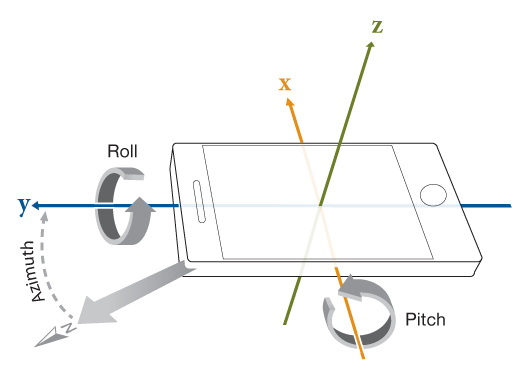
\includegraphics[width=8.5cm]{phoneOrientation}
	\caption{Orientation for a mobile phone}\label{FIG_1}
\end{figure}


\section{Technical Approach}

Find the geoframe orientation of the PowerDue and mobile phone

\subsection{Compute attitude of device}

The phone attitude is obtained by doing continuos integration on the angular
velocity, and by taking the difference between the geo-framea, the earth
coordinate sytem, and the body-frame, the coordinate system of the device's
body. Per \cite{PhoneAttitude}, the best approach for calculating the difference
between both coordinate systems is the Euler Axis/Angle method, which solves the
problem from the geo-frames perspective. To compute the integration, the total
device motion is split into multiple time windows, and the rotation of the
device is the accumulated rotation of all the time windows.

\subsection{Madgwick}

Historically, the Kalman filter, and other techniques, including fuzzy
processing and frequency domain filters, have been used as the basis for
orientation algorithms; however, these techniques have several disadvantages
\cite{Madgwick}. For example, the Kalma filter requires is computationally
expensive, and some of the other techniques are only effective under limited
conditions \cite{Madgwick}. Therefore, we plan to use Madgwick, an algorithm
that employs a quaternion representation of orientation, which has had positive
results despite the fact that it does not require the heavy computational load,
or high sampling frequency, of a Kalman-filter based algorithm \cite{Madgwick}.

\section{Plan of Attack}

\begin{enumerate}
\item Obtain a sensor with a gyroscope and accelerometer.
\item Write the code for a driver, if necessary.
\item Compute the attitude of the PowerDue.
\item Compute the attidue of a mobile phone.
\item Correlate the readings from the PowerDue and mobile phone.
\end{enumerate}

\section{Conclusion}

Conclusion.

% References

\bibliographystyle{Bibliography/IEEEtranTIE}
\bibliography{Bibliography/IEEEabrv,Bibliography/BIB_1x-TIE-2xxx}\ %IEEEabrv instead of IEEEfull

{\color{red}

\vspace{-1cm}
\begin{IEEEbiography}[{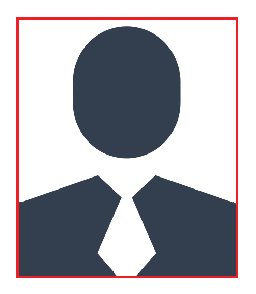
\includegraphics[width=1in,height=1.25in,clip,keepaspectratio]{photo-men.eps}}]
{First A. Author1} and the other authors may include biographies at the end of regular papers. The first paragraph may contain a place and/or date of birth (list place, then date). Next, the author's educational background is listed. The degrees should be listed with type of degree in what field, which institution, city, state or country, and year degree was earned. The author's major field of study should be lower-cased.

The second paragraph uses the pronoun of the person (he or she) and not the author's last name. It lists military and work experience, including summer and fellowship jobs. Job titles are capitalized. The current job must have a location; previous positions may be listed without one. Information concerning previous publications may be included.

The third paragraph begins with the author's title and last name (e.g., Dr. Smith, Prof. Jones, Mr. Kajor, Ms. Hunter). List any memberships in professional societies other than the IEEE. Finally, list any awards and work for IEEE committees and publications. If a photograph is provided, the biography will be indented around it. The photograph is placed at the top left of the biography. Personal hobbies will be deleted from the biography.
\end{IEEEbiography}

\vspace{-2cm}
\begin{IEEEbiography}[{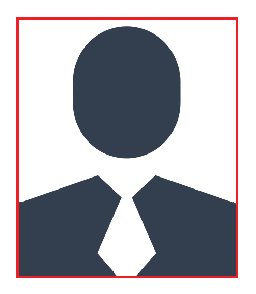
\includegraphics[width=1in,height=1.25in,clip,keepaspectratio]{photo-men.eps}}]
{Second B. Author2} (M'12) was born in City, Country. He received the M. degree in electrical engineering from University of City, Country in 2012.

The second paragraph uses the pronoun of the person (he or she) and not the author's last name. It lists military and work experience, including similar information to the previous author, including military, work experience, and other jobs. Job titles are capitalized. The current job must have a location; previous positions may be listed without one. Information concerning previous publications may be included.

The third paragraph begins with the author's title and last name (e.g., Dr. Smith, Prof. Jones, Mr. Kajor, Ms. Hunter), including similar information to the previous author, including the list of any awards and work for IEEE committees and publications. The photograph is placed at the top left of the biography. Personal hobbies will be deleted from the
biography.\\
\end{IEEEbiography}

\vspace{-2cm}
\begin{IEEEbiography}[{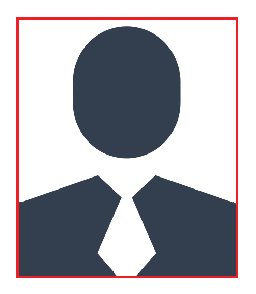
\includegraphics[width=1in,height=1.25in,clip,keepaspectratio]{photo-men.eps}}]
{Third C. Author3} (M'99-SM'04-F'09) was born in City, Country. He received the M. and SM. and F. degrees in electrical engineering from University of City, Country in 1999, 2004 and 2009 respectively.

The second paragraph uses the pronoun of the person (he or she) and not the author's last name. It lists military and work experience, including similar information to the previous author, including military, work experience, and other jobs.

The third paragraph begins with the author's title and last name (e.g., Dr. Smith, Prof. Jones, Mr. Kajor, Ms. Hunter), including similar information to the previous author, including the list of any awards and work for IEEE committees and publications. The photograph is placed at the top left of the biography. Personal hobbies will be deleted from the biography.
\\ \\
\end{IEEEbiography}

}

\end{document}
